\documentclass{article}

\usepackage{amsmath, amsfonts, geometry, palatino, mathpazo,
graphicx}

%%%%%%%%%%%%%%%%%%%%%%%%%%%%%%%%%%%%%%%%%%%%%%%%%%%%%%%%%%%%%%%
\newenvironment{proof} {\textbf{Proof:} \newline} {\hfill
  $\mathcal{Q.E.D.}$}

\newenvironment{thm}[2][]{\vspace{0.2cm} \textbf{Theorem #2:
    \textit{#1}} \newline}{}

\newenvironment{defn}[2][]{\vspace{0.2cm} \textbf{Definition #2:
    \textit{#1}} \newline}{}
%%%%%%%%%%%%%%%%%%%%%%%%%%%%%%%%%%%%%%%%%%%%%%%%%%%%%%%%%%%%%%%


\begin{document}

\title{An Introduction to Bayes' Theorem}
\author{Joyce Tipping}
\date{}
\maketitle

\setlength{\parindent}{0cm}
\setlength{\parskip}{0.3cm}

\section{Preliminary Remarks}

A few preliminary definitions and theorems will make Bayes'
Rule easy to derive.

\subsection{Conditional Probability}

First, we will define conditional probability. The following
definition and theorem are reversed in some textbooks; that
is, the theorem is given as the definition and vice
versa. Since one implies the other, it really hardly
matters.

\begin{defn}[Conditional Probability]{1}
  The conditional probability of an event $A$, given the event
  $B$, is defined by $$P(A|B) = \frac{P(A \cap B)}{P(B)}$$ if
  $P(B) \neq 0$.
\end{defn}


\begin{thm}[Multiplication Theorem]{1}
  For any events $A$ and $B$, $$P(A \cap B) = P(A|B)P(B) =
  P(B|A)P(A).$$
\end{thm}

\begin{proof}
    Since $P(A|B) = \frac{P(A \cap B)}{P(B)}$, it follows
    that $P(A \cap B) = P(A|B)P(B)$.

    Notice that since $P(A \cap B) = P(B \cap A)$ and
    $P(B|A) = \frac{P(B \cap A)}{P(A)}$, we have $P(A \cap
    B) = P(B|A)P(A)$.

\end{proof}

Remember that, intuitively, the probability that an event
$A$ happened is simply the number of ways $A$ can happen
divided by the total number of scenarios.

With this in mind, the definition of Conditional Probability
should make sense upon closer inspection. When we say $A$
given $B$, we are saying that $B$ already happened. Thus, we
restrict our sample space to $B$. Then, the probability that
$A$ happened is simply the probability of $A \cap B$ over
the probability of $B$.

The Multiplication Theorem follows algebraically from the
Law of Conditional Probability.

\begin{figure}
\centering
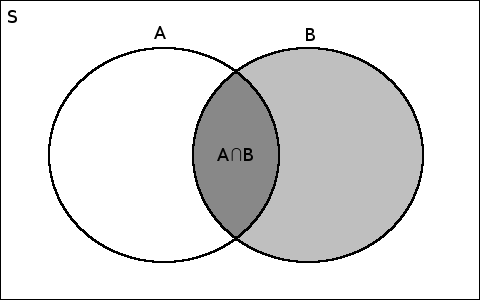
\includegraphics[height=2in,
width=3.2in]{fig-1-conditional-probability.png}
\caption{The Law of Conditional Probability}
\end{figure}
  
\subsection{Total Probability}

\begin{thm}[Total Probability]{2}
  If $B_1, ..., B_k$ is a collection of mutually exclusive and
  exhaustive events, then for any event $A$, $$P(A) =
  \sum_{i=1}^k P(B_i)P(A|B_i)$$
\end{thm}

\begin{proof}
  The events $A \cap B_1, A \cap B_2, \ldots, A \cap B_k$
  are mutually exclusive, so it follows that $$P(A) =
  \sum_{i=1}^k P(A \cap B_i).$$ The theorem results from
  applying the Theorem 1 to each term in this summation.
\end{proof}

The Law of Total Probability, while nasty in notation, is
really not so bad. It is best thought of as putting together
a jigsaw puzzle. For example, in Figure 2, the total
probability of $A$ is the sum of the ``pieces,'' the
probabilities of $A$ intersected with each $B_i$.

\begin{figure}
\centering
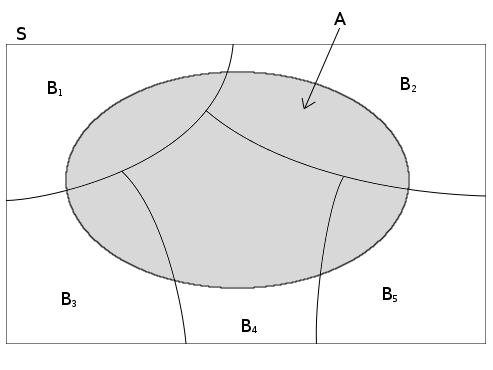
\includegraphics[width=3in,
height=2.25in]{fig-2-total-probability.png}
\caption{The Law of Total Probability}
\end{figure}

  
\section{Bayes' Rule}

Bayes' Rule is really a compendium of the previous
concepts. The proof follows almost trivially from these
results.

\begin{thm}[Bayes' Rule]{3}
  If $B_1, ..., B_k$ is a collection of mutually exclusive and
  exhaustive events, then for each $j = 1, ..., k$, $$P(B_j|A) =
  \frac{P(B_j)P(A|B_j)}{\sum_{i=1}^k P(B_i)P(A|B_i)}$$
\end{thm}

\begin{proof}
  From Definition 1 and the Multiplication Theorem, we have

  $$P(B_j|A) = \frac{P(A \cap B_j)}{P(A)} =
  \frac{P(B_j)P(A|B_j)}{P(A)}$$

  The result follows by applying Theorem 2 to the
  denominator.
\end{proof}


\section{Example}
Scientists have developed a new medical test for a very rare
disease. Only 0.1\% of the population has this disease. When
a patient has the disease, the test correctly returns a
positive result 99\% of the time. However, if a patient does
not have the disease, the test returns a false positive 5\%
of the time.

Suppose a patient has tested positive. What is the
probability that he has the disease?

\vspace{0.5cm}
\textbf{Answer:}
Define the following events:

\quad $D$ = Patient has disease

\quad $D'$ = Patient does not have disease

\quad $T$ = Test returns a positive

\quad $T'$ = Test returns a negative


We know that a randomly selected patient has a 0.001 prior
probability of having the disease: $P(D) = 0.001$.

We also are given that given a patient has the disease, the
test returns positive 99\% of the time: $P(T|D) = 0.99$.

Finally, if a patient does not have the disease, the test
returns a false positive 5\% of the time: $P(T|D') = 0.05$.

Our question is, if a patient tests positive, what is the
probability he has the disease?: Find $P(D|T)$.

By the definition of conditional probability, we have
\begin{eqnarray*}
P(D|T) &=& \frac{P(D \cap T)}{P(T)}\\
&=& \frac{P(T|D)P(D)}{P(T \cap D) + P(T \cap D')}\\
&=& \frac{P(T|D)P(D)}{P(T|D)P(D) + P(T|D')P(D')}\\
&=& \frac{0.05 \cdot 0.001}{0.05 \cdot 0.001 + 0.99 \cdot
  0.999}\\
&=& 0.019
\end{eqnarray*}

Interpretation: When the test returns positive, the patient
actually has the disease only 1.9\% of the time. In other
words, the test returns a false positive 98.1\% of the time.

A tree diagram is helpful for understanding problems that
are a series of steps, at each of which there are one or
more choices. Figure 3 shows the tree diagram for this
problem. Notice that the probabilities on the second layer
are conditional probabilities, and that each set of branches
emanating from a common point sum to 1.

\begin{figure}[h]
\centering
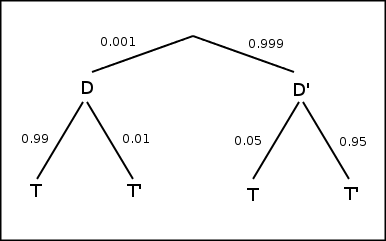
\includegraphics[height=2in, width=3.2in]{fig-3-ex-tree.png}
\caption{Tree Diagram}
\end{figure}

Since we've been representing things with Venn diagrams so
far, it might seem disorienting to go to a tree diagram all
of the sudden. Figure 4 shows the same situation represented
with a Venn diagram. As you can see, it is a good deal
harder to understand.

\begin{figure}[h]
\centering
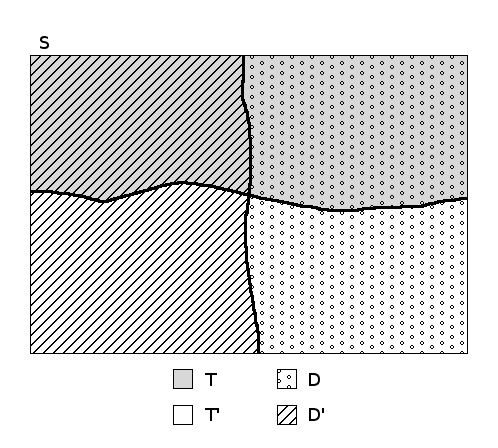
\includegraphics[height=3.15in, width=3.5in]{fig-4-ex-venn.png}
\caption{Venn Diagram}
\end{figure}
  
\end{document}